\documentclass[a4paper]{jpconf}
\usepackage{graphicx}

\begin{document}
\title{Systematic profiling to monitor and specify the software refactoring process of the LHCb experiment}

\author{Ben Couturier}
\address{CERN, CH-1211 Geneva 23, Switzerland}
\ead{ben.couturier@cern.ch}

\author{Emmanouil Kiagias}
\address{CERN, CH-1211 Geneva 23, Switzerland}
\ead{emmanouil.kiagias@cern.ch}

\author{Stefan B. Lohn}
\address{CERN, CH-1211 Geneva 23, Switzerland}
\ead{stefan.lohn@cern.ch}

\begin{abstract}
The LHCb collaboration develops and maintains large software frameworks, critical to the good performance of the experiments, that face challenges due to the increase of throughput requested from the Physics side that will not be matched by the computing resources, and by new computing architectures such as many-core, that cannot be currently fully used due to the limited amount of memory available per core. In the coming years, a considerable refactoring effort will therefore be needed to vectorize and parallelize the code, to minimize hotspots and to reduce the impact of bottlenecks. It is crucial to guide the refactoring with a profiling system that gives hints to parts for possible and necessary source-code re-engineering and which kind of optimization could lead to final success.
\newline
Software optimization is a sophisticated process where all parts, compiler, operating system, libraries and chosen hardware play a role in. Intended improvements can have different effects on different platforms. To obtain precise information of the general performance, to make profiles comparable, reproducible and to verify the progress of performance in the framework, it is important to produce profiles more systematically in terms of regular profiling based on representative use cases and to perform regression tests. Once a general execution, monitoring and analysis platform is available, software metrics can be derived from the collected profiling results to trace changes in performance back and to create summary reports on a regular basis with an alert system if modifications led to significant performance degradations.
\end{abstract}

\section{Introduction}
\label{sec:introduction}

In large scale software solutions of high energy physics, performance is critical for efficient result extraction. Plenty of profiling tools are available and must be integrated to trace performance already from an early state in development. But often software is more evolving because of considerations of maintainability, usability, flexibility, due to necessary features implementation or urgent bug fixes, than due to performance optimization. Often it appears, that such information are not clearly and reliable available to determine the importance of performance optimizing measures. Hence, performance has less or no priority, also because there are no information about certain software behavior at all. The LHCb performance \& regression (PR) project tries to address this issue for the LHCb experiment at CERN to allow more intervention which relies on performance information.    
\newline
During its development phase, the LHCb software was constantly optimized; the profiling was however in responsibility of each developer, with no ``official'' profiling test suite defined and no record of the results. While this approach was effective in the framework development phase, there are no record of the evolution in software performance, nor of the current baseline. With a refactoring of the code under way it is therefore now necessary for LHCb to put systematic profiling tests in place, in order to ensure that there is no performance degradation.
\newline
This paper describes the LHCb PR framework, to profile the experiments software and to display results in a user friendly manner. This paper describes an overview about LHCb software and the objectives of the LHCb PR project in chapter \ref{sec:lhcb_computing}, the work-flow with some implementation aspects in chapter \ref{sec:workflow_and_implementation} and briefly goes into upcoming challenges in chapter \ref{sec:lhcbpr_and_beyond}.

\section{LHCb computing}
\label{sec:lhcb_computing}

\subsection{LHCb software}
\label{sec:lhcb_software}

The LHCb experiment software is based on Gaudi\cite{gaudi}, a C++ framework using generic and object-oriented features of C++ for computing intensive tasks, and python for configuring and structuring modules (algorithms, tools...). The application manager executes consecutive an abstract series of algorithms to process data objects from the transient store on request. Gaudi is providing core services and tools for applications to hide complexity and make future development and changes more transparent for users. It is a large-scale framework and is additionally used by ATLAS, Glast, Harp and other experiments.
\newline
Applications build on top of Gaudi are Moore, Brunel, DaVinci, Gauss, Boole and others. Moore is the implementation of the High-Level Trigger (HLT) to decide weather event data will be stored or not, Brunel is responsible for the offline reconstruction of tracks, DaVinci is the physics analysis framework, Gauss to simulate the particle transport and interaction through several detector modules, and Boole performs the digitization.

\subsection{Computing environment}
\label{sec:computing_environment}

The LHCb computing environment persists out of the computing resources accessed in the Worldwide LHC Computing Grid (WLCG), in Cloud Infrastructure and in the HLT farm located at the experiment. Additional, virtualization is used and just recently volunteer computing has been added. Some 100k CPU's are involved in the data processing. 
%35 GB/s of recorded data have to be processed by 1500 computing nodes of the Event Filtering Farm (EFF) of the HLT to be reduced to 70 MB/s \cite{lhcb_hlt_opt}.

\subsection{Integrated Profiling}
\label{sec:integrated_profiling}

In HEP computing it is a common method to measure performance via throughput (events processed per time unit). Thus the performance analysis is focused on the time linear and not the time constant part of processing. Instrumentation is an important advantage for profiling source-code in large scale frameworks like the applications from the LHCb experiment. Multiple profiling measures have been implemented in the Gaudi framework using the AuditorService \cite{status_gaudi} which provides an interface for executing code between events or algorithms processed.
\newline
Timing information from the operating system's process information are collected using the TimingAuditor and are printing a summary of time spend in the applications algorithms. Likewise information can be collected using the Memory- or MemStatAuditor for changes in memory as soon as they appear. Recent work \cite{intel_auditor} conducted by Mazurov and Couturier shows how to improve precision in profiling the event-loop using instrumentation routines of Intel's VTune\texttrademark Amplifier API, which can be added using the IntelAuditor. Another strategy is to collect information from the performance monitoring unit (PMU) of modern CPU architectures to collect information about hardware usage and issues such as cache-misses, branch-misprediction and more as done by Kruse and Kruzelecki \cite{modular_monitoring} for the Gaudi framework. Many of such kind of work has been performed to provide tools for developers to profile their code. Still, systematic usage or comparative profiling has been sparsely observed.

\subsection{Systematic Profiling}
\label{sec:integrated_profiling}

Three important aspects must be considered as crucial for systematic profiling. Profiles must become \textit{comparable}, \textit{reproducible} and \textit{representative} to allow regression analysis and to trace back changes in performance to source-code locations. For a series of regular profiles for several platforms, profiling must be limited to a small number of default cases and a fixed set of reference data. Reference data are also important to avoid variance due to different types of physics. This way differences in execution behavior between two revisions can be examined and traced back on changes in related source-code. On the other side, changing the reference set of physics events could later on be used to evaluate the needs of computing resources for upcoming data-taking periods and changing recorded event information.
%Systematic profiling should not only trace back hotspots and drawbacks of changes in code, but shell help to obtain and understanding which techniques, tool for optimization, or changing platforms are having a higher impact on saving computing resources.
\newline
Furthermore, profiles must be reproducible to be able to compare the test configuration of executed test jobs. This affects the job configuration, to log the software/platform information, as well as the run configuration provided by option files for Gaudi applications. Finally, gathered information should be precise and reliable making a regular execution of a series of test jobs necessary.
\newline
Hence the LHCb PR project has the following requirements.
\begin{enumerate}
 \item The expected huge amount of information must be centrally collected and easily become accessible. This can be achieved by using a web application as interface to support brief analysis of collected data.
 \item Profiling is a changing subject with new interesting technologies. A solution must be flexible to include new profiling tools. Information must be collected by parsing generated reports and hooking them onto a central database.
 \item To reduce work generic ways of navigation and visualization have to be investigated by trying to use supporting tools as much as available.
 \item Regular execution would be labor intensive without an automated execution chain. Automated triggering, setup and data collection of the profiling procedure simplifies systematic profiling attempts.
\end{enumerate}
To fulfill the objectives and requirements, the LHCb PR project contains three important technical aspects. First, the PRConfig project was created to store the run configuration in a version control system and to collect further job information and final profiling results into a central SQL database. Second, Jenkins \cite{jenkins} a continuous integration system is used to configure, trigger and submit test jobs and finally Django \cite{django} to support the web application to quickly visualize and propagate results. 

\begin{figure}{t}
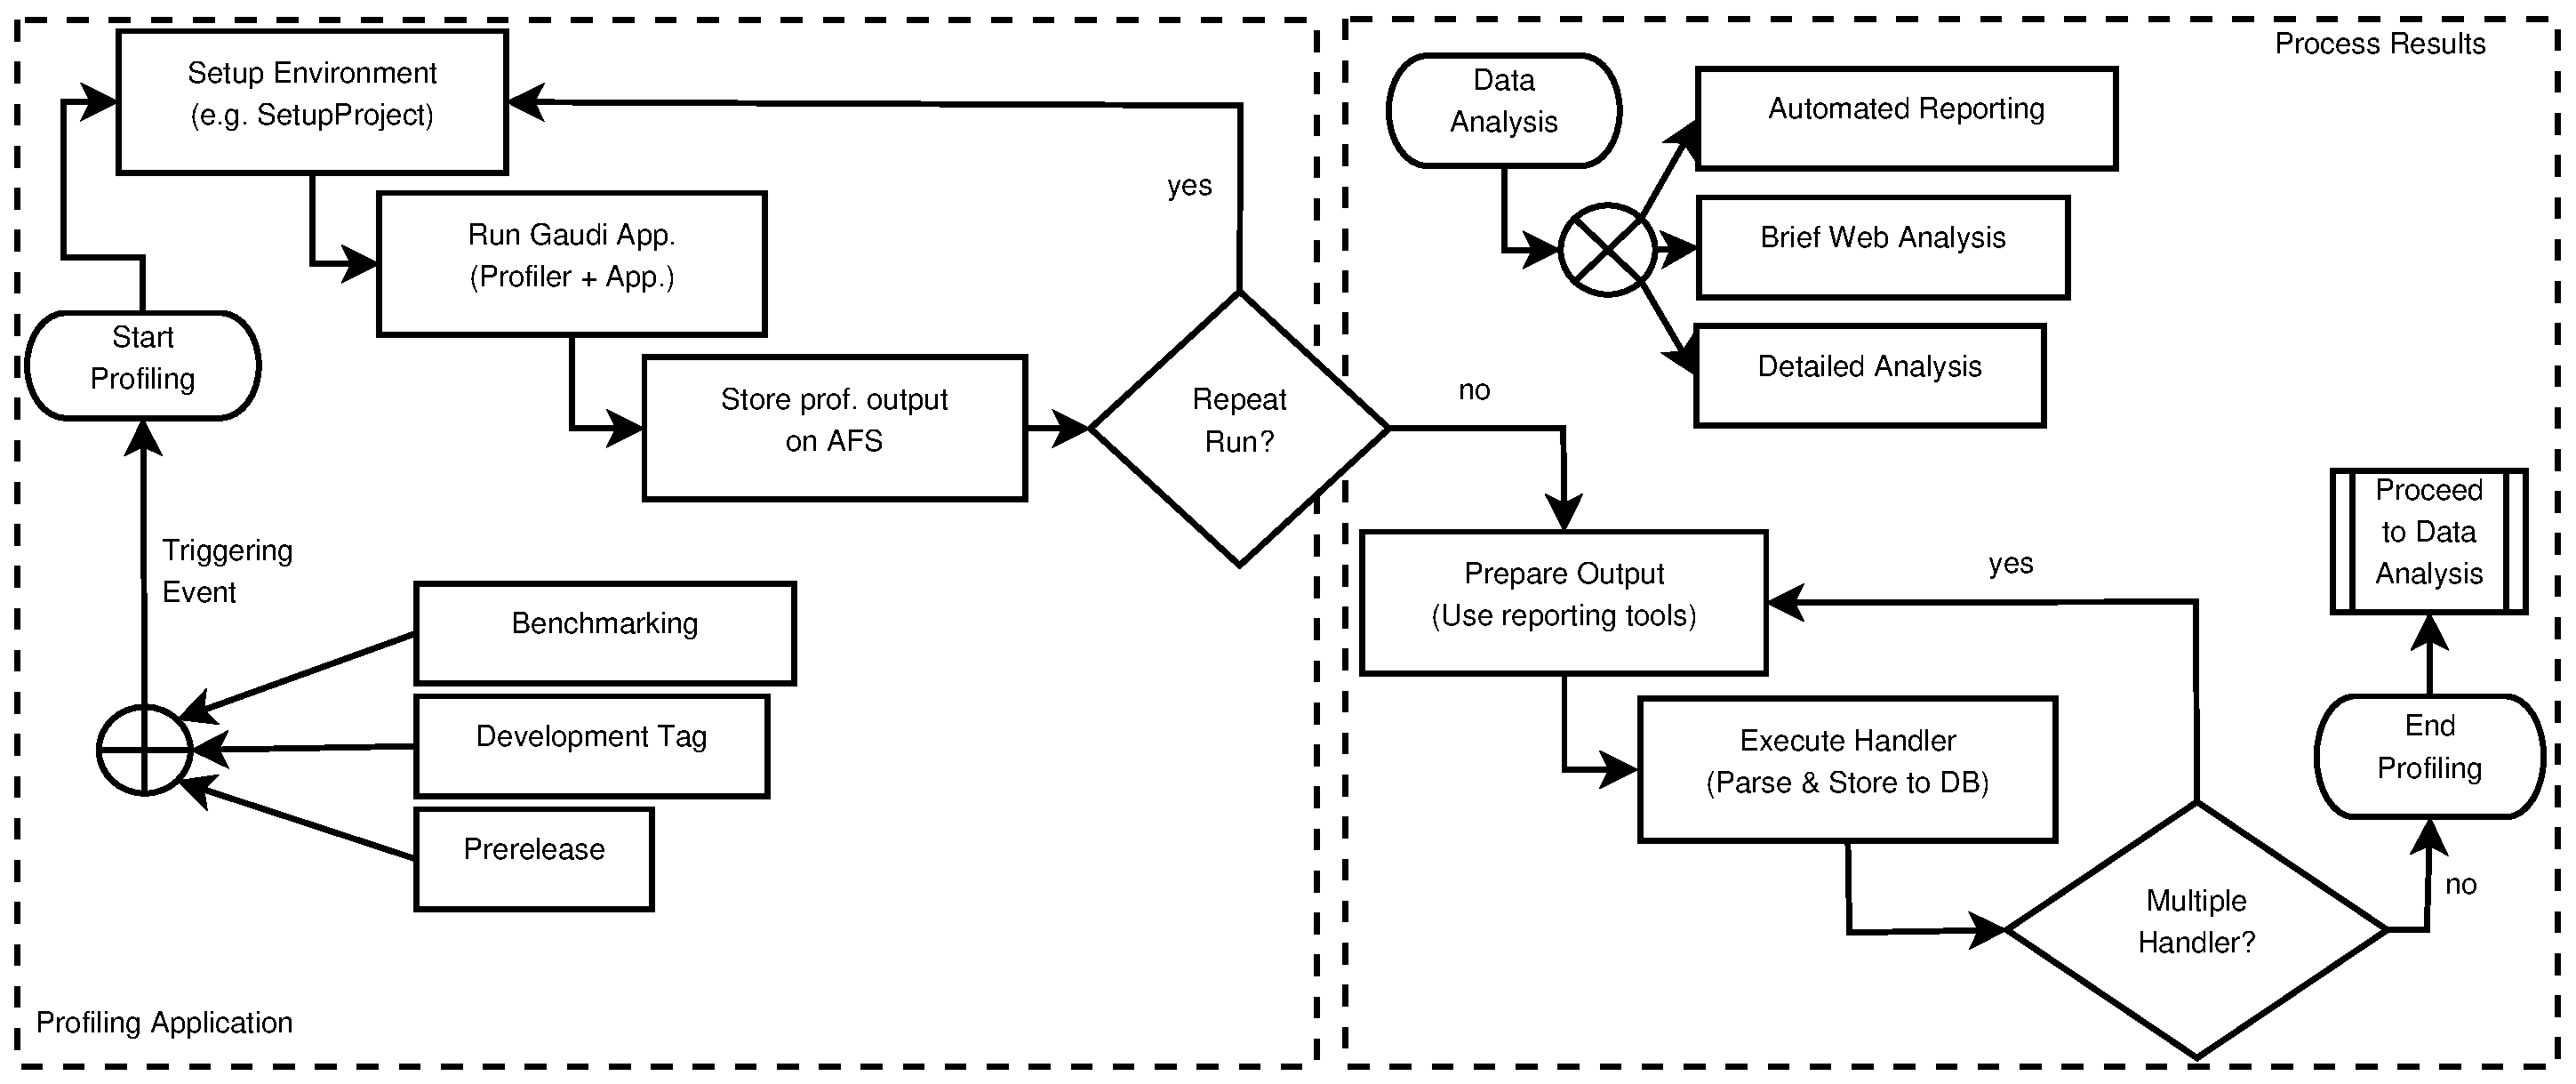
\includegraphics[scale=0.3]{figures/profiling_process.eps}
\caption{\small \textit{The profiling procedure includes three stages. First, the test definition, triggering and submission. Second, the run execution, repetition and data collection by using data handlers to parse profiling reports and send core information to the database. And third, quick access to gathered profiling results by generating summary reports, using a web application for quick access to compare the general performance or to access detailed profile collected during the run.}}
\label{fig:profiling_process}
\end{figure}

\section{Work-flow and Implementation}
\label{sec:workflow_and_implementation}

The LHCb PR project provides support to conduct systematic profiling. The work-flow of a test execution is summarized in \mbox{figure \ref{fig:profiling_process}}, where Jenkins is used to configure, trigger and schedule test jobs before profiling. While execution, a profiler specific wrapper is downloaded and used to hide the profiler specific call for Jenkins and to setup the test environment for multiple executions. While execution, profiler information is gathered on a remote network file system for later detailed analysis. In the end, data handlers to parse reports and collect results are called, which are defined for distinct types of profiles and some additional job information like comments, files and classes of setups. Depending on the desired information, profiles can be filtered or combined with other available information. Then, results are hooked onto a SQL database. In the end the LHCb PR web analysis framework facilitates profile comparisons and helps detecting anomalies in performance.

\subsection{LHCb PR framework}
\label{sec:lhcbpr_framework}

The core of the LHCb PR framework is a customized analysis interface based on Django. The backbone of Django is based on python to speed up development while keeping a certain amount of flexibility due to a variety of auxiliary modules available. Additionally, processing intensive tasks can be performed on the server-side while keeping the interface quick and smart.
\newline
LHCb PR can ruffly be divided into two main aspects, navigation and visualization. Plotting graphs is current done by using visualization capabilities of the ROOT framework and its python interface pyRoot or using Google Charts. Different kinds of analysis are referring to different ways of visualization in which data attributes, as generic items for performance information, are shown. For instance, the Basic-Analysis shows the distribution of attributes, the Trend shows the progress of attributes cross versions or revisions and the Overview-Analysis about several attributes between a few versions or platforms. Attributes can be runtime, resident memory, possibly lost memory or even more complex software performance or quality metrics.
\newline
For a top-down analysis, the Trend has been added to observe changes cross revisions and versions to figure out progress in performance. Significant changes become immediately conspicuous, but requires single attributes, e.g. one of many algorithms, to be tracked. A better observation of several attributed is allowed by the Overview. Both show entries with their statistical variance, but to get precise information about the distribution around their average, the Basic-analysis is indispensable using ROOT histograms.
\newline
To navigate easily through data, results can directly accessed by their category, a tuples of job description id, platform and host. To select categories, a generic selection menu allows to specify categories for comparison.  The generic menu is amended by customized part to specify profiling groups (profiling information), attributes or filtering options important to the specific visualization. Data access is also available on job level via a job table accessible through a table of different test configurations or categories.

\subsection{Job distribution and triggering}
\label{sec:job_distribution}

To facilitate regular profiling in a series of equal tests to permit statistic evaluations, Jenkins helps to manage the job distribution to test hosts. It makes the inclusion of further hosts simple and prevents interferences between multiple jobs running on the same machine by avoiding over-commitment. Test configurations can be prepared by creating parametrized jobs in the Jenkins interface. Test specific preparations, e.g. compiling packages (software modules) with specific compiler flags, can be added depending on the use case.
\newline
Despite configuring jobs, cron jobs in Jenkins can be used for triggering a profiling procedure within the release- or build cycle. This way, from triggering to execution and data collection, no human intervention is necessary, what simplifies data collection and opens the way to point out reliable and significant changes in the software profile.

%\subsection{Execution and Profiling}
%\label{sec:execution_and_profiling}

%Commercial and open-source profilers becoming more and more usable. The open source community developed crucial tools like the valgrind tool suit. Other tools like google's tcmalloc can be used to elaborate processing time and memory consumption. Additional, recent hardware features give access to hardware counters of the PMU (performance monitoring unit), which can be read from proprietary software like intels VTune or open source projects like oprofile.
%\newline
%This paper is not going to evaluate the benefits and drawbacks of different tools, but wants to enable a profiling platform like LHCb PR to individually setup these tools on their specific way. For these purposes scripts are collected into a separate repository which can easily execute the test cases and stay flexible for an individual configuration. To improve the configuration of profiling runs and to focus the profiling onto main time consuming parts, integration of the profilers instrumentation methods are highly recommended.

\subsection{Data collection}
\label{sec:data_collection}

Data collection can be handled in three different ways, first one can segregate information from results to be stored in the database, second, files which contain performance information can be made available for downloading on the web-interface and third, bigger profiles can become available on remote storage. Segregating information from different profilers can be addressed by several parsers or data handler for each different profiling report. To maintain flexibility for many kinds of different profiling tasks, the post-processing of profiling must prepare parsable reports. The LHCbPR handler project attempts to collect these data. It further transfers information about the other, not parsed, profiling data for further examinations.

\begin{figure}[t]
\begin{minipage}[t]{17pc}
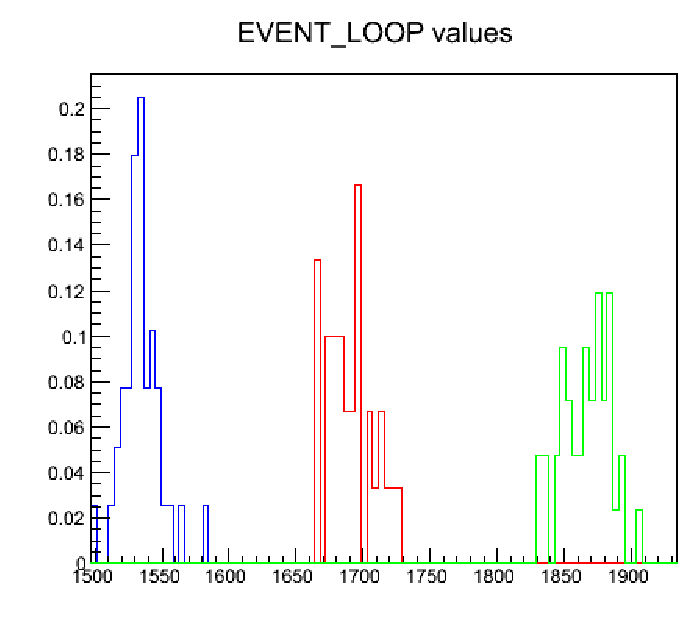
\includegraphics[scale=0.55]{figures/brunel_basic_libm.eps}
\caption{\small \textit{Runtime distribution of a Brunel version using different glibc's ([ms] per event) of the event\_loop attribute for different math libraries. (blue) Intel, (red) elder libm, (green) updated libm of a new glibc version.}}
\label{fig:brunel_basic_libm}
\end{minipage}\hspace{1pc}
\begin{minipage}[t]{17pc}
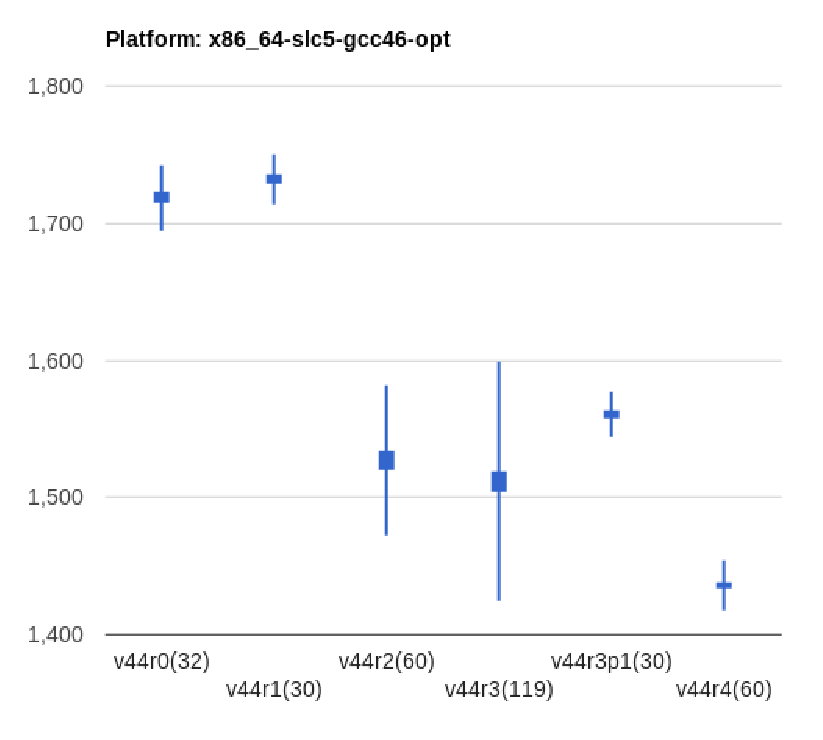
\includegraphics[scale=0.48]{figures/brunel_trend_analysis.eps}
\caption{\small \textit{Trend analysis of Brunel to monitor changes cross versions.}}
\label{fig:brunel_trend}
\end{minipage}
\end{figure}

\subsection{Test cases}
\label{sec:test_cases}

Use cases are important to trace performance changes back to the evolving algorithms. Test cases shell base on default use cases for best approximations to the production usage. Still, the sophisticated computing environments can influence runs on a non-predictive non-deterministic way, which hampers conclusions from regression analysis. Currently, the highest priority is to find software related issues, that can be addressed or have to be taken into account for upcoming decisions in resource allocation.
\newline
Default cases for Brunel have been quickly evaluated, defined and are running now on a regular basis after each successful build. LHCb PR has demonstrated its importance already by observing simple timing information obtained by the TimingAuditor. Significant changes become immediately clear by observing the trend information cross versions as shown exemplary in figure \ref{fig:brunel_trend}. After observing performance degradation further tests using the IntelAuditor have shown, that performance changes were once originated in external math libraries, as shown in Figure \ref{fig:brunel_basic_libm}. VTune\texttrademark can now be used for regular runs to visualize runtime spent in libraries and algorithms.
\newline
Unfortunately the HLT framework Moore can not simply be reduced to a view common default cases, what makes it more difficult to trace back performance issues using a top-down analysis. The HLT brings further complications for the PR project in two main aspects:
\begin{enumerate}
 \item The computing environment at the HLT farms are highly sophisticated with processes cloned to run multiple processes on the same job, with events coming ...
 \item Single or a few default cases, as required, are not available because of constantly changing trigger configuration keys (TCKs), which define the algorithms involved.
\end{enumerate}
The first problem, as discussed, can not fully be addressed. First, more default cases can be used for a closer approximation and second, a standard configuration can be defined to make the analysis, as applied for Brunel, available. The second problem, can partially be addressed by not only splitting use cases, but also the software into parts for further investigations. This would also simplifies tracing back performance issues to source-code locations to help particular software development efforts. 

\section{LHCb PR and beyond}
\label{sec:lhcbpr_and_beyond}

\subsection{Profiling accuracy}
\label{sec:profiling accuracy}

In the current state, the web-interface does not provide a resolution beyond algorithm level. More detailed information are currently only accessible with the collected profile information profilers like Valgrind or VTune. The resolution of the interface is limited for two good reasons. First, developer shell be provided with profiles but competing with the variety of visualization tools of highly sophisticated profilers is unreasonable difficult and second, a tremendous amount of data that would have to be collected and stored. Still it could be reasonable to increase the resolution to function level. This becomes at latest with Moore evident, because algorithms are not executed in a strict order and for access to certain services lazy initialization is used. For instance tracking in the vertex detector is started by the first algorithm which requests these information and later on data can directly be accessed. This makes algorithm vary in their profile, what can currently not be reasonable traced back from the web analysis.

\subsection{Complementary information}
\label{sec:complementary_information}

Due to the issue of the latter paragraph, the unordered execution of algorithms need to be addressed. This can be done by adding further complementary information, like a function call-stack for each algorithm to give a much higher resolution for finding anomalies in profiles than currently available, and it would make profiles of algorithms more comprehensive.
\newline
Another upcoming task is that if once a test case is fully implemented to be analyzed by several profilers in distinct runs, and if much more general information are available, these information could also be used to be correlated to each other. This way it would be possible to find the impact of design decisions and to validate existing methods or new concepts. Then open questions could be answered as knowledge base for further developments.
\newline
At the moment measurements like CPI, cache-misses, branch-misprediction and others are often mentioned, but can barely be correlated to real performance influences. Questions like how much exactly the call-stack depth influences runtime by occurring more cache-misses, and how does this influences current R\&D project like Gaudi-Hive by sharing cache among threads could then be emphasized by concrete numbers.

\begin{figure}[t]
\begin{minipage}[b]{0.33\textwidth}
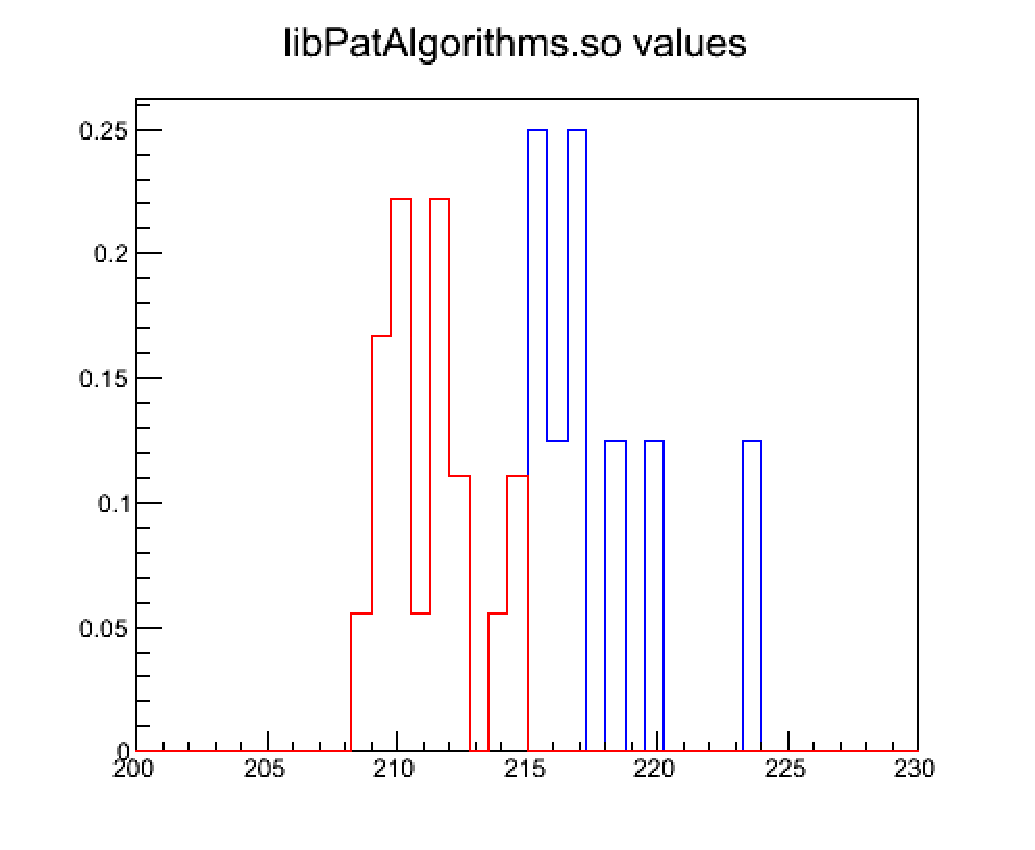
\includegraphics[scale=0.3]{figures/moore_basic_vect.eps}
\caption{\small \textit{Comparing auto-vectorized library in Moore again unvectorized version.}}
\label{fig:moore_basic}
\end{minipage}\hspace{0.5cm}%
\begin{minipage}[b]{0.60\textwidth}
\centering
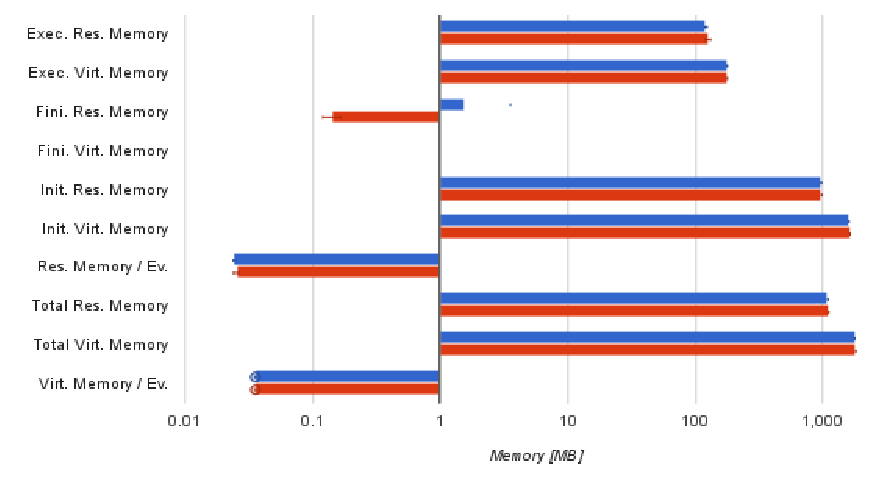
\includegraphics[scale=0.50]{figures/moore_overview_memory.eps}
\caption{\small \textit{For some application memory consumption is crucial. An overview of several memory information to observe differences between version.}}
\label{fig:moore_overview}
\end{minipage}
\end{figure}

\section{Conclusions}
\label{sec:conclusions}

Using a flexible, extensible and customizable platform to collect and summarize profiling results enables the LHCb collaboration to systematically compare profiles. The LHCb PR project has already demonstrated to be highly valuable. Performance due to changing software and advancing technology could be observed, examined and appropriately be addressed. Since implementing instrumentation is in many aspects already performed, since many profilers can be applied for data collection and since Django and Jenkins is reducing the necessary work to set up a performance monitoring system, the effort is absolutely affordable for large scale projects as those from the LHCb collaboration. Still, improvements have to be discussed and put into place, but due to the easy adaptivity to the web interface and testing framework, more and more fields for application, like including software metrics into testing and analysis become tangible. 
%This is organized in a way that takes additional tasks away from developers and simplifies the profiling to introduce a certain level of automation, e.g. for performance validation before a new release. It permits an arbitrary level of flexibility due to including new profilers and to monitor new software performance and quality values. The web front-end simplifies the task of monitoring the general performance of the Gaudi frameworks applications. 

\section*{References}
\bibliographystyle{iopart-num}
\begin{thebibliography}{9}
\bibitem{gaudi} G. Corti, M. Cattaneo, P. Charpentier, M. Frank, P. Koppenburg, P. Mato, F. Ranjard, S. Roiser, I. Belyaev and G. Barrand, {\it ``Software for the LHCb experiment''}, IEEE Transactions on Nuclear Science, vol. 53, nb. 3, P.1323-1328, 2006
\bibitem{status_gaudi} P. Mato and others, {\it ``Status of the GAUDI event-processing framework''}, Intl. conference on computing in high energy and nuclear physics, Beijing, China, 2001
\bibitem{lhcb_hlt_opt}M. Frank, C. Gaspar, E. v Herwijnen, B. Jost, N. Neufeld, and R. Schwemmer, {\it ``Optimization of the HLT Resource Consumption in the LHCb Experiment''}, J. Phys.: Conf. Ser. 396 012021, 2012
\bibitem{intel_auditor} A. Mazurov and B. Couturier, {\it ``Advanced Modular Software Performance Monitoring''}, J. Phys.: Conf. Ser. 396 052054, 2012
\bibitem{modular_monitoring} D. F. Kruse and K. Kruzelecki, {\it ``Modular Software Performance Monitoring''}, J. Phys.: Conf. Ser. 331 042014, 2011
\bibitem{django} ``Django is a high-level Python Web framework'', url: https://www.djangoproject.com/
\bibitem{jenkins} ``Jenkins, An extendable open source continuous integration server'', url: https://www.jenkins-ci.org/
\end{thebibliography}
\end{document}
